\documentclass[12pt]{article}
\usepackage{preamble}

\pagestyle{fancy}
\fancyhead[LO,LE]{Физические основы компьютерных \\ и сетевых технологий}
\fancyhead[CO,CE]{30.09.2024}
\fancyhead[RO,RE]{Лекции Музыченко Я. Б.}

\fancyfoot[L]{\scriptsize исходники найдутся тут: \\ \url{https://github.com/pelmesh619/itmo_conspects} \Cat}

\begin{document}
    \section{4.
    Импульс. Закон сохранения импульса.}

    \begin{tcolorbox}[colframe=blue!25, colback=blue!10, title=\textbf{План лекции}]

        \footnotesize
        \begin{itemize}
            \item Силы в механике

            \item Универсальные законы природы - законы сохранения

            \item Импульс материальной точки

            \item Закон сохранения импульса

            \item Центр масс. Ц-система
        \end{itemize}
    \end{tcolorbox}

    \subsection{Силы в механике. Сила гравитационного взаимодействия}

    Все силы в механике относятся к гравитационным и электромагниным фундаментальным воздействиям.
    Это можно заметить на примере законов всемирного тяготения и Кулона:

    \begin{multicols}{2}
        \begin{center}
            $\vec{F} = G \frac{m_1 m_2}{r^3_{12}} \vec{r}_{12}$

            Закон всемирного тяготения
        \end{center}

        \begin{center}
            $\vec{F} = k \frac{q_1 q_2}{r^3_{12}} \vec{r}_{12}$

            Закон Кулона
        \end{center}
    \end{multicols}

    Запишем закон всемирного тяготения для тела $m$ на расстоянии $r$ от Земли (радиуса $R$ и массы $M_{\text{З}}$):

    \[|\vec{F}| = G\frac{mM_{\text{З}}}{(R + r)^2}\]

    С другой стороны, любое тело вблизи поверхности Земли движется с ускорением свободного падения $\vec{g}$, следовательно,
    сила, действующая на тело, равна:

    \[F = G\frac{mM_{\text{З}}}{R^2} = mg\]

    Одинаково ли ускорение свободного падения на поверхности Земли? % жопа

    \smallvspace

    \begin{minipage}{\textwidth}
        \begin{wrapfigure}{r}{0pt}
            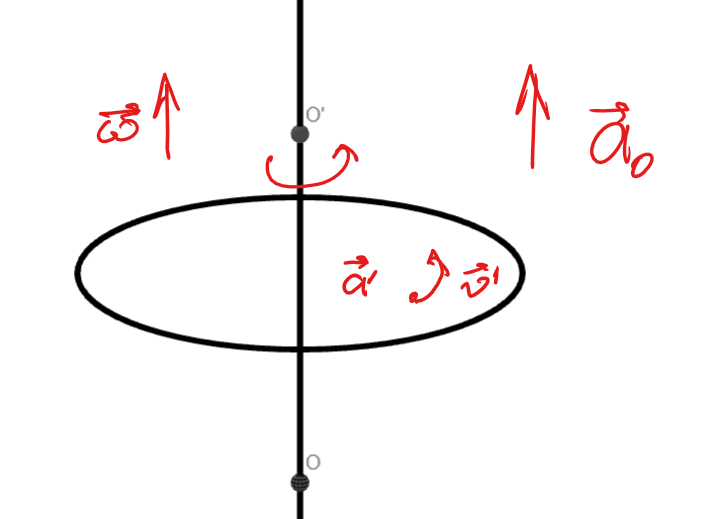
\includegraphics[height=5cm]{physics1/images/physics1_2024_09_30_1}
        \end{wrapfigure}

        Пусть $k$ - ИСО, $k^\prime$ - НИСО (неинерциальная СО), а $\vec{a}^\prime, \vec{v}^\prime$ - ускорение и скорость в системе $k^\prime$,
        а сама система $k^\prime$ движется с ускорением $\vec{a_0}$ и вокруг оси с угловой скоростью $|\vec{\omega}| = const$


        Тогда получаем ускорение в НИСО: $\vec{a}^\prime = \vec{a} + \omega^2 \vec{\rho} + 2 [\vec{v}^\prime \vec{\omega}] - \vec{a}_0$

        $\vec{a}$ - ускорение тела в системе $k^\prime$

        $\omega^2 \vec{\rho}$ - центробежное ускорение

    \end{minipage}

    \smallvspace

    $2 [\vec{v}^\prime \vec{\omega}]$ - ускорение Кориолиса

    $\vec{a}_0$ - поступательное ускорение (системы отсчета $k^\prime$ для $k$)

    $m\vec{a}^\prime = \underset{\sum \vec{F}}{\underbrace{m\vec{a}}} + \underset{\text{силы инерции (т. н. фиктивные)}}{\underbrace{m\omega^2 \vec{\rho} + 2m [\vec{v}^\prime \vec{\omega}] - m\vec{a}_0}}$ - основное уравнение динамики в НИСО

    $m \omega^2 \vec{\rho}$ - центробежная сила

    $2m [\vec{v}^\prime \vec{\omega}]$ - сила Кориолиса

    $m\vec{a}_0$ - поступательная сила инерции


    В НИСО возникают так называемые силы инерции (фиктивные), центробежная и Кориолиса связаны с вращением

    Сила Кориолиса будет действовать только на те тела, которые движутся

    Из закона всемирного тяготения можно вывести ускорение свободного падения гравитационное: $g_{\text{грав}} = G \frac{M_\text{З}}{R^2} = 9.81\dots9.83 \frac{\text{м}}{\text{с}^2}$

    Из этого получить ускорение эффективное: $g_\text{эфф} = g_\text{грав} + a_\text{цб} = 9.78\dots9.83$ (ускорение свободного падения уменьшается на 3 сотых из-за вращения)

    \subsection{Вес тела}

    \Def Вес тела - сила, с которой тело действует на неподвижную относительно него опору

    В случае опоры $|P| = |N|$ ($N$ - сила реакции опоры)

    Рассмотрим случай, когда тело находится в неподвижном состоянии на поверхности:

    $m\vec{g} + \vec{N} = 0 \quad\quad N - mg = 0 \quad\quad P = mg$

    Вес тела равен силе тяжести только при $\vec{a} = 0$ системы отсчета

    \subsection{Силы трения}

    Силы трения появляются при перемещении соприкасающихся тел или их частей относительно друг друга.
    Различают сухое и вязкое трение. К сухому трению относится трение покоя, трение скольжения и трение качения

    \textbf{Сила трения покоя} применима не телам, которые покоятся; она не может превышать некоторого максимального значения: $0 \leq F_\text{тр.} \leq \mu_0 N$ (где $\mu_0$ - коэффициент трения покоя)

    \textbf{Сила трения скольжения} возникает при движении соприкасающихся тел. В общем случае сила трения скольжения зависит
    от скорости движения, но для широкого класса тел равна максимальной силе трения покоя и подчиняется закону Амонтона-Кулона: $F_\text{тр} = \mu N$

    В задачах принимается, что $\mu_0 = \mu$, тогда во время покоя сила трения растет линейно, пока не достигнет $\mu N$, тогда тело начинает движение, и применяется сила трения скольжения

    \subsection{Как можно измерить массу тел?}

    Для измерения массы необходимо сравнить ее с другой, принятой за эталон. Сравним массы $m_1$ и $m_2$

    Опыт показывает, что в замкнутой системе - системе, в которой можно пренебречь взаимодействием с другими телами,
    выполняется соотношение:

    $\frac{\Delta \vec{v}_1}{\Delta \vec{v}_2} = \frac{m_2}{m_1}$

    $\Delta \vec{v}_1 \uparrow \downarrow \Delta \vec{v}_2 \quad\quad\quad v \ll c$

    $m_1 \Delta \vec{v}_1 = -m_2 \Delta \vec{v}_2$ или $m_1 \Delta \vec{v}_1 + m_2 \Delta \vec{v}_2 = 0$

    Импульс (количество движения) - векторная величина, равная произведению массы тела на его скорость: $\vec{p} = m\vec{v} \quad\quad [p] = \text{кг} \cdot \text{м/с}$

    Определение справедливо для материальной точки и для поступательного движения твердого тела

    Импульс системы материальных точек: $\vec{P} = \sum_{i = 1}^N \vec{p}_i$

    Для системы $N$ материальных точек ($\vec{F}_i$ - внешние силы)

    $\frac{d\vec{P}}{dt} = \sum \vec{F}_i \quad\quad\quad \vec{P} = const$

    Закон сохранения импульса - импульс замкнутой системы остается постоянным


    При изменении состояния системы всегда существуют такие величины, которые сохраняются с течением времени. Среди этих величин наиболее важное значение имеют импульс, энергия и момент импульса.

    Эти величины обладают свойством аддитивности – значение величин для системы, состоящей из частей, равно сумме значений для каждой из частей в отдельности.

    Законы сохранения – универсальные законы природы, связаны с фундаментальными свойствами пространства и времени.

    \begin{center}
        Закон сохранения импульса – однородность пространства

        Закон сохранения энергии – однородность времени

        Закон сохранения момента импульса – изотропность пространства
    \end{center}

\end{document}
